\documentclass[nonumber]{homework}
\usepackage{enumitem}

\newcommand{\hwclass}{Math 6108}
\newcommand{\hwname}{Jacob Hauck}
\newcommand{\hwtype}{Homework}

\newcommand{\R}{\textbf{R}}
\newcommand{\dee}{\;\text{d}}
\newcommand{\eps}{\varepsilon}
\newcommand{\pl}[2]{\frac{\partial #1}{\partial #2}}
\newcommand{\dl}[2]{\frac{\text{d} #1}{\text{d} #2}}
\newcommand{\sgn}{\text{sgn}}
\newcommand{\bigoh}{\mathcal{O}}

\newcommand{\hwnum}{6}

\usepackage{listings}
\usepackage{graphicx}
\usepackage{caption}
\usepackage{subcaption}


\begin{document}
	\maketitle
	
	\question*{3.2}
	Let $a \in \R$, and consider the difference equation
	\begin{equation*}
		x_{n+1} = f(x_n) = \frac{2}{3}x_n + \frac{a}{3x_n^2}.
	\end{equation*}
	Then $f$ has only one fixed point equal to $\sqrt[3]{a}$ because
	\begin{equation*}
		f(x) = x \implies x = \frac{2}{3}x + \frac{a}{3x_n^2} \implies x^3 = a \implies x = \sqrt[3]{a}.
	\end{equation*}
	Furthermore, $\sqrt[3]{a}$ is an asymptotically stable fixed point because
	\begin{equation*}
		f'(\sqrt[3]{a}) = \frac{2}{3} - \frac{2a}{3a} = 0. 
	\end{equation*}
	Using the script in Listing \ref{lst:cbrt_sim} (see appendix), we see that it takes about 4 iterations starting from an initial guess of 1.5 for the first 5 digits to settle down -- see the console output in Listing \ref{lst:3.2}.
	
	\begin{lstlisting}[basicstyle=\small\ttfamily, frame=single, caption={Console command and output}, label=lst:3.2]
> python -m cbrt 2 --guess 1.5
n = 0    x_n = 1.5

n = 1    x_n = 1.2962962962962963

n = 2    x_n = 1.2609322247417485

n = 3    x_n = 1.2599218605659261

n = 4    x_n = 1.2599210498953948
	\end{lstlisting}
	
	\newpage
	
	\question*{Euler method for $\sqrt{2}$ with a large step size}
	We would like to consider the difference equation
	\begin{equation*}
		x_{n+1} = x_n - h\frac{x_n^2 - 2}{2x_n},
	\end{equation*}
	which is Euler's method for approximating $\dot{x} = -\frac{x^2-2}{2x}$ with step size $h > 0$. For the right step size, this method should converge to $\sqrt{2}$. We have already seen that this works with $h = 1$. Using the script in Listing \ref{lst:euler} (see appendix) we see that the method also appears to converge with $h = 1.5$ and $h = 1.9$ but fails to converge with $h = 2.5$ and $h = 2.1$ --  see Listings \ref{lst:step1.5}, \ref{lst:step1.9}, \ref{lst:step2.1}, \ref{lst:step2.5} for the corresponding console output.
	
	\begin{minipage}{\linewidth}
	\begin{lstlisting}[basicstyle=\small\ttfamily, frame=single, caption={Console command and output, $h=1.5$ (abridged)}, label=lst:step1.5]
>python -m euler --start 1.6 --step 1.5
x_0 = 1.6

x_1 = 1.3375

x_2 = 1.4558703271028037

x_3 = 1.3942791226290783

...

x_11 = 1.414134600476956

x_12 = 1.4142530466279473

x_13 = 1.4141938210724339
	\end{lstlisting}
	\end{minipage}
	
	\begin{lstlisting}[basicstyle=\small\ttfamily, frame=single, caption={Console command and output, $h=1.9$ (abridged)}, label=lst:step1.9]
>python -m euler --start 1.6 --step 1.9
x_0 = 1.6

x_1 = 1.2674999999999998

x_2 = 1.5623888067061145

x_3 = 1.2942059815629339

...

x_97 = 1.4142072829470977

x_98 = 1.4142192138829808

x_99 = 1.4142084760356535	
	\end{lstlisting}
	
	\begin{minipage}{\linewidth}
	\begin{lstlisting}[basicstyle=\small\ttfamily, frame=single, caption={Console command and output, $h=2.1$ (abridged)}, label=lst:step2.1]
>python -m euler --start 1.6 --step 2.1
x_0 = 1.6

x_1 = 1.2324999999999997

x_2 = 1.6422289553752538

x_3 = 1.1966383837491845

x_4 = 1.6950842096270753

...

x_18 = 3.0776930236495614

x_19 = 0.5284446077342535

x_20 = 3.9475042119776256

x_21 = 0.33460648903505996
	\end{lstlisting}
	\end{minipage}
	
	
	\begin{minipage}{\linewidth}
		\begin{lstlisting}[basicstyle=\small\ttfamily, frame=single, caption={Console command and output, $h=2.5$ (abridged)}, label=lst:step2.5]
>python -m euler --start 1.6 --step 2.5
x_0 = 1.6

x_1 = 1.1624999999999996

x_2 = 1.8599126344086028

x_3 = 0.8791709985946473

x_4 = 2.623795134842801

...

x_66 = 0.08931453285309976

x_67 = 27.968636780129696

x_68 = -6.902773358330645

x_69 = 1.363520069474804
		\end{lstlisting}
	\end{minipage}
	
	\newpage
	
	\question*{3.4 (a)}
	
	Consider the parametric map
	\begin{equation*}
		f(\lambda, x) = \lambda x(1-x)
	\end{equation*}
	for $\lambda > 1$. This map has fixed points when
	\begin{equation*}
		x = \lambda x(1-x) \implies x(\lambda x + 1-\lambda) = 0,
	\end{equation*}
	so when $x = x_1 = 0$ or $x = x_2 = 1 - \frac{1}{\lambda}$. To find when these equilibrium points are non-hyperbolic, we need to find $\lambda > 1$ such that $|f_x(\lambda, x_i)| = 1$, where $i = 1,2$. 
	
	Since $f_x(\lambda, x) =\lambda(1-2x)$, we see that $x_1$ is non-hyperbolic if $|\lambda| = 1$, which is impossible under the constraint $\lambda > 1$, so $x_1$ is always hyperbolic.
	
	On the other hand, $x_2$ is non-hyperbolic if 
	\begin{equation*}
		|\lambda(1-2x_2)| = \left|\lambda\left(1 - 2+\frac{2}{\lambda}\right)\right| = 1 \iff |2-\lambda| = 1,
	\end{equation*}
	that is, when $\lambda =1$ or when $\lambda = 3$. Since we are considering $\lambda > 1$, we see that $x_2$ is non-hyperbolic only when $\lambda =3$.
	
	To determine the stability of $x_1$ and $x_2$, we observe that $|f_x(\lambda, x_1)| = |\lambda| > 1$, so $x_1$ is always unstable. For $x_2$, observe that $|f_x(\lambda, x_2)| = |2-\lambda|$. Since $|2-\lambda| < 1$ is equivalent to $1 < \lambda < 3$, we see that $x_2$ is asymptotically stable if $\lambda < 3$. Since $|2-\lambda| > 1$ is equivalent to $\lambda < 1$ or $\lambda>3$, we see that $x_2$ is unstable if $\lambda > 3$.
	
	To investigate the stability of $x_2$ when $\lambda = 3$, we turn to the stair-step diagrams in Figure \ref{fig:3.4a}. Apparently, $x_2$ is asymptotically stable when $\lambda = 3$ (see Figure \ref{fig:3.4aeq3}). 
	
	Diagrams were generated using the code in Listing \ref{lst:stairstep}.
	
	\begin{figure}[h]
		\begin{subfigure}{.33\textwidth}
			\centering
			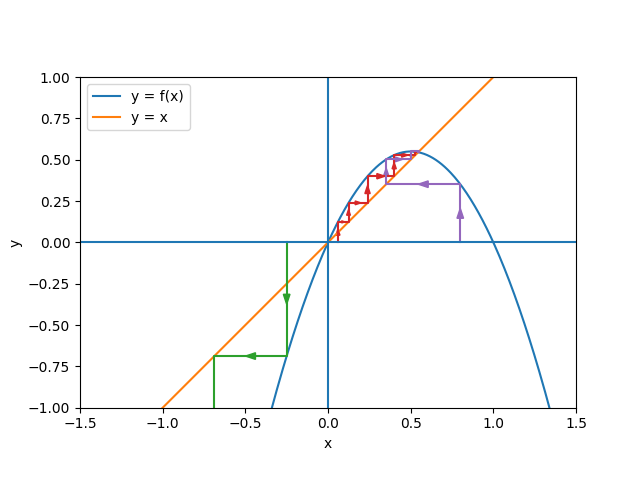
\includegraphics[width=\linewidth]{3.4a lambda lt 3.png}
			\caption{$\lambda < 3$}
			\label{fig:3.4alt3}
		\end{subfigure}
		\begin{subfigure}{.33\textwidth}
			\centering
			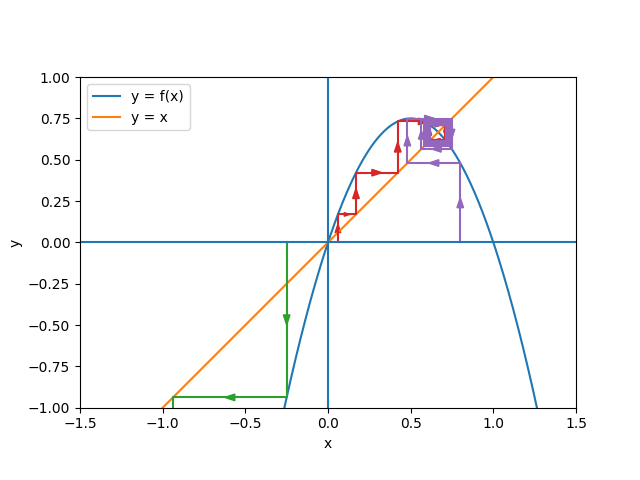
\includegraphics[width=\linewidth]{3.4a lambda eq 3.png}
			\caption{$\lambda = 3$}
			\label{fig:3.4aeq3}
		\end{subfigure}
		\begin{subfigure}{.33\textwidth}
			\centering
			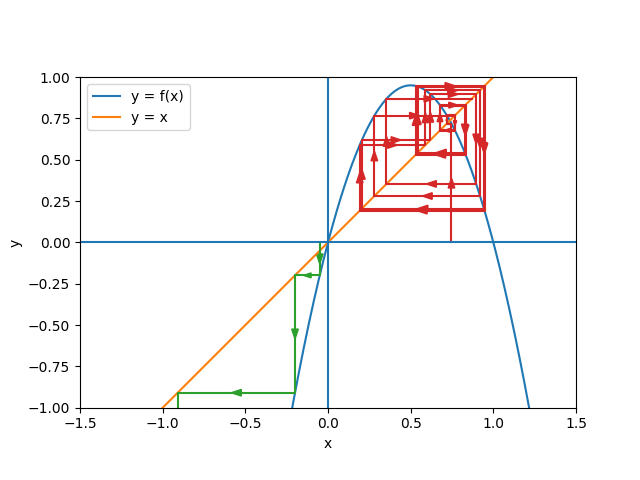
\includegraphics[width=\linewidth]{3.4a lambda gt 3.png}
			\caption{$\lambda > 3$}
			\label{fig:3.4agt3}
		\end{subfigure}
		\caption{3.4 (a) typical stair-step diagrams}
		\label{fig:3.4a}
	\end{figure}
	
	\newpage
	
	\question*{3.4(c)}
	Consider the parametric map
	\begin{equation*}
		f(\lambda, x) = \lambda - x^2.
	\end{equation*}
	This map has fixed points when
	\begin{equation*}
		\lambda - x^2 = x \iff x^2 + x - \lambda = 0,
	\end{equation*}
	so when
	\begin{equation*}
		x = x_1 = \frac{-1 + \sqrt{1 + 4\lambda}}{2} \qquad\text{or}\qquad x = x_2 = \frac{-1-\sqrt{1+4\lambda}}{2}.
	\end{equation*}
	This can only occur if $\lambda \ge -\frac{1}{4}$; otherwise, there are no fixed points. In the special case that $\lambda = -\frac{1}{4}$, we see that $x_1 = x_2 = -\frac{1}{2}$ and there is actually only one fixed point.
	
	Noting that $f_x(\lambda, x) = -2x$, we If $\lambda = -\frac{1}{4}$, then the fixed point $-\frac{1}{2}$ is non-hyperbolic because
	\begin{equation*}
		\left|f_x\left(-\frac{1}{4}, -\frac{1}{2}\right)\right| = 1.
	\end{equation*}
	
	If $\lambda > -\frac{1}{4}$, then we can determine the values of $\lambda$ such that the two fixed points $x_1$ and $x_2$ are non-hyperbolic by setting $|f_x(\lambda, x_i)| = 1$ for $i = 1,2$. Starting with $x_2$, we see that
	\begin{equation*}
		|f_x(\lambda, x_2)| = |-2x_2| = 1 + \sqrt{1+4\lambda} > 1,
	\end{equation*}
	so $x_2$ is always hyperbolic. For $x_1$, we see that
	\begin{equation*}
		|f_x(\lambda, x_1)| = |-2x_1| = \left|1-\sqrt{1+4\lambda}\right| = 1 \iff \sqrt{1+4\lambda} = 0 \quad\text{or}\quad \sqrt{1+4\lambda} = 2.
	\end{equation*}
	The former is impossible because we are considering the case that $\lambda > -\frac{1}{4}$, and $\sqrt{1+4\lambda} = 2$ if and only if $1 + 4\lambda = 4$, that is, $\lambda = \frac{3}{4}$. Thus, $x_2$ is non-hyperbolic only when $\lambda = \frac{3}{4}$.
	
	To determine the stability of the fixed points, we first consider $x_2$ when $\lambda > -\frac{1}{4}$, as this fixed point is always hyperbolic. We see that
	\begin{equation*}
		|f_x(\lambda, x_2)| = 1 + \sqrt{1+4\lambda} > 1
	\end{equation*}
	regardless of the value of $\lambda > -\frac{1}{4}$, so $x_2$ is always unstable.
	
	Next, we consider $x_1$ when $\lambda > -\frac{1}{4}$ and $\lambda \ne \frac{3}{4}$. We have
	\begin{equation*}
		|f_x(\lambda, x_1)| = \left|1-\sqrt{1+4\lambda}\right| < 1 \iff 0 < \sqrt{1 + 4\lambda} < 2.
	\end{equation*}
	The last inequalities are equivalent to $-\frac{1}{4} < \lambda < \frac{3}{4}$, so $x_1$ is stable when $\lambda < \frac{3}{4}$. If $\lambda > \frac{3}{4}$, then certainly $|f_x(\lambda, x_1)| > 1$, so $x_1$ is unstable when $\lambda > \frac{3}{4}$.
	
	To investigate the stability of the hyperbolic fixed points $-\frac{1}{2}$ when $\lambda = -\frac{1}{4}$ and $x_2$ when $\lambda = \frac{3}{4}$, we turn to the stair-step diagrams in Figure \ref{fig:3.4c}. We see that $-\frac{1}{2}$ when $\lambda = -\frac{1}{4}$ appears to be unstable (see Figure \ref{fig:3.4ceq-14}), and $x_2$ when $\lambda = \frac{3}{4}$ appears to be asymptotically stable (see Figure \ref{fig:3.4ceq34}).
	
	Diagrams were generated using the code in Listing \ref{lst:stairstep}.
	
	
	\begin{figure}[h]
		\begin{subfigure}{.33\textwidth}
			\centering
			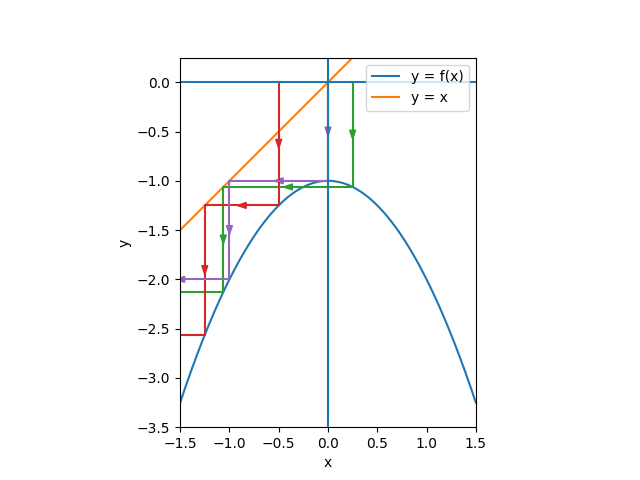
\includegraphics[width=\linewidth]{3.4c lambda lt -14.png}
			\caption{$\lambda < -\frac{1}{4}$}
			\label{fig:3.4clt-14}
		\end{subfigure}
		\begin{subfigure}{.33\textwidth}
			\centering
			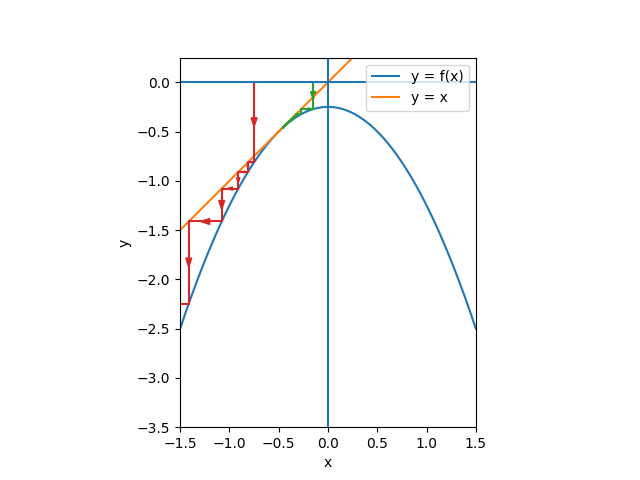
\includegraphics[width=\linewidth]{3.4c lambda eq -14.png}
			\caption{$\lambda = -\frac{1}{4}$}
			\label{fig:3.4ceq-14}
		\end{subfigure}
		\begin{subfigure}{.33\textwidth}
			\centering
			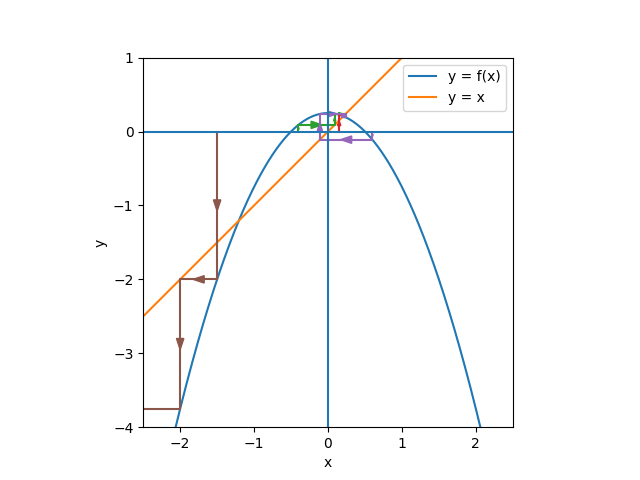
\includegraphics[width=\linewidth]{3.4c lambda gt -14.png}
			\caption{$-\frac{1}{4} < \lambda < \frac{3}{4}$}
			\label{fig:3.4cgt-14}
		\end{subfigure}
		\begin{subfigure}{.33\textwidth}
			\centering
			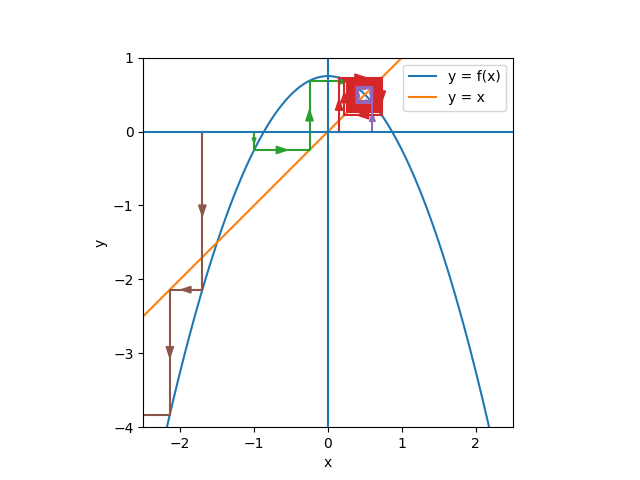
\includegraphics[width=\linewidth]{3.4c lambda eq 34.png}
			\caption{$\lambda = \frac{3}{4}$}
			\label{fig:3.4ceq34}
		\end{subfigure}
		\begin{subfigure}{.33\textwidth}
			\centering
			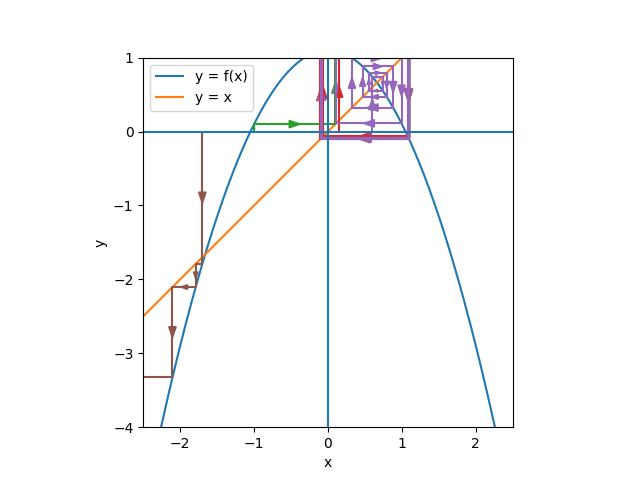
\includegraphics[width=\linewidth]{3.4c lambda gt 34.png}
			\caption{$\lambda > \frac{3}{4}$}
			\label{fig:3.4cgt34}
		\end{subfigure}
		\caption{3.4 (c) typical stair-step diagrams}
		\label{fig:3.4c}
	\end{figure}
	
	\clearpage
	\newpage
	\mbox{}
	
	\question*{3.4(d)}
	
	Consider the parametric map
	\begin{equation*}
		f(\lambda, x) = \lambda^2 - x^2.
	\end{equation*}
	This map is effectively the same as the one in 3.4(c) but reparametrized with $\lambda^2$ in place of $\lambda$. Since $\lambda^2 > -\frac{1}{4}$ for any value of $\lambda$, we can recycle the calculations from 3.4(c) to find that the fixed points of $f$ are
	\begin{equation*}
		x_1 = \frac{-1 + \sqrt{1+4\lambda^2}}{2} \qquad\text{and}\qquad x_2 = \frac{-1-\sqrt{1+4\lambda^2}}{2}.
	\end{equation*}
	Further recycling calculations from 3.4 (c), the fixed point $x_1$ is always hyperbolic and unstable, and the fixed point $x_2$ is non-hyperbolic only when $\lambda^2 = \frac{3}{4}$, that is, when $\lambda = \pm \frac{\sqrt{3}}{2}$. Additionally, $x_2$ is asymptotically stable if $\lambda^2 < \frac{3}{4}$, that is, if $|\lambda| < \frac{\sqrt{3}}{2}$, and $x_2$ is unstable if $\lambda^2 > \frac{3}{4}$, that is, if $|\lambda| > \frac{\sqrt{3}}{2}$. Finally, $x_2$ is also asymptotically stable if $\lambda^2 = \frac{3}{4}$, that is, if $\lambda = \pm\frac{\sqrt{3}}{2}$.
	
	Stair-step diagrams for these different cases are given in Figure \ref{fig:3.4d}. Diagrams were generated using the code in Listing \ref{lst:stairstep}.
	
	\begin{figure}[h]
		\begin{subfigure}{.33\textwidth}
			\centering
			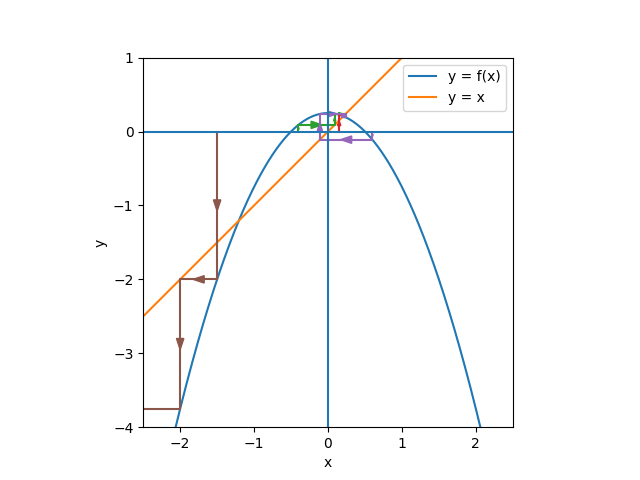
\includegraphics[width=\linewidth]{3.4d lambda lt sqrt(3)2.png}
			\caption{$|\lambda| < \frac{\sqrt{3}}{2}$}
			\label{fig:3.4dlt}
		\end{subfigure}
		\begin{subfigure}{.33\textwidth}
			\centering
			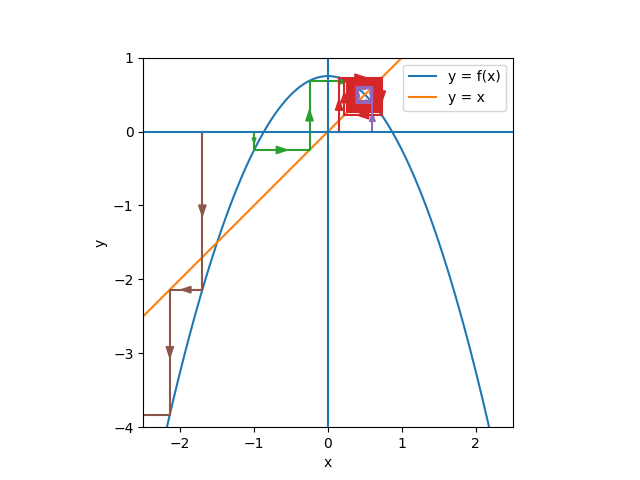
\includegraphics[width=\linewidth]{3.4d lambda eq sqrt(3)2.png}
			\caption{$|\lambda| = \frac{\sqrt{3}}{2}$}
			\label{fig:3.4deq}
		\end{subfigure}
		\begin{subfigure}{.33\textwidth}
			\centering
			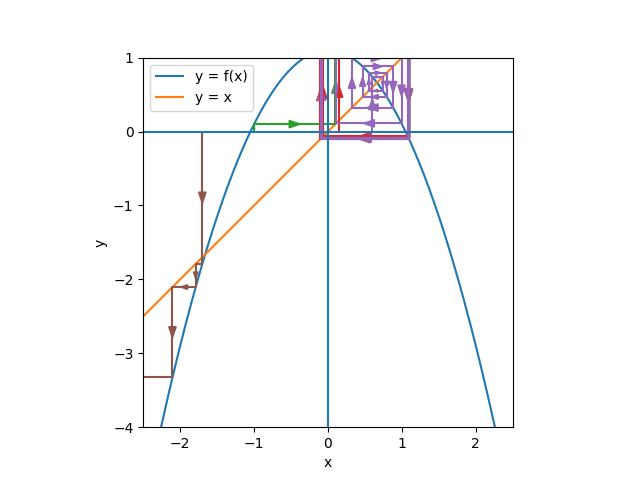
\includegraphics[width=\linewidth]{3.4d lambda gt sqrt(3)2.png}
			\caption{$|\lambda| > \frac{\sqrt{3}}{2}$}
			\label{fig:3.4dgt}
		\end{subfigure}
		\caption{3.4 (d) typical stair-step diagrams}
		\label{fig:3.4d}
	\end{figure}
	
	\newpage
	
	\question*{3.6}
	
	Consider the map
	\begin{equation*}
		x_{n+1} = f(x_n) = bx_n\left(\frac{1+b}{b} - x_n\right).
	\end{equation*}
	This map has fixed points when
	\begin{equation*}
		x = f(x) = bx\left(\frac{1+b}{b} - x\right) \iff bx(1-x) = 0,
	\end{equation*}
	so when $x = 0$ or $x = 1$. Note that
	\begin{equation*}
		f'(x) = 1+b - bx -bx = 1 + b - 2bx
	\end{equation*}
	Then $0$ is asymptotically stable when $|1+b| < 1$, that is, when $-2 < b < 0$, and $0$ is unstable when $|1+b| > 1$, that is, when $b < -2$ or $b > 0$.
	
	Furthermore, $1$ is asymptotically stable when $|1-b| < 1$, that is, when $0 < b < 2$, and $1$ is unstable when $|1-b|> 1$, that is, when $b < 0$ or $b > 2$.
	
	When $b = -2$ or $2$, at least one of the fixed points is non-hyperbolic, and we turn to the stair-step diagrams in Figure \ref{fig:3.6} to determine stability (note that we don't mind about $b=0$ because the map requires us to divide by $b$, so we must assume $b\ne0$). From the stair-step diagrams, we see that $0$ is asymptotically stable when $b = -2$ (see Figure \ref{fig:3.6eq-2}), and $1$ is asymptotically stable when $b = 2$ (see Figure \ref{fig:3.6eq2}).
	
	Diagrams were generated using the code in Listing \ref{lst:stairstep}.
	
	\begin{figure}[h]
		\begin{subfigure}{.33\textwidth}
			\centering
			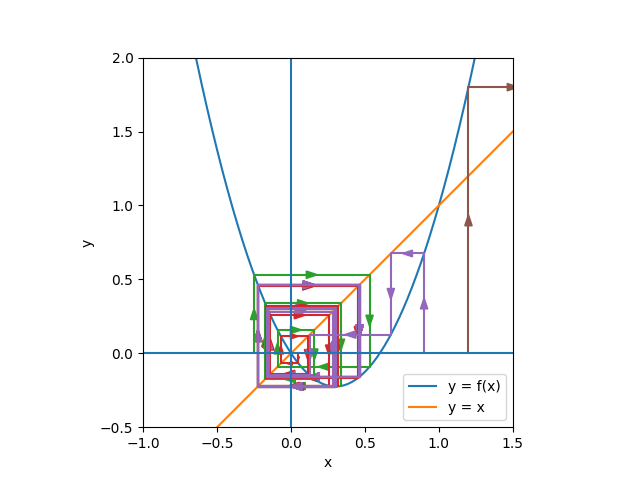
\includegraphics[width=\linewidth]{3.6 b lt -2.png}
			\caption{$b < -2$}
			\label{fig:3.6lt-2}
		\end{subfigure}
		\begin{subfigure}{.33\textwidth}
			\centering
			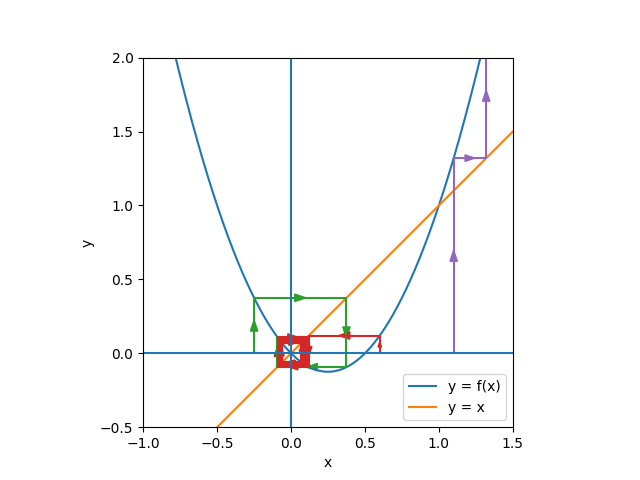
\includegraphics[width=\linewidth]{3.6 b eq -2.png}
			\caption{$b = -2$}
			\label{fig:3.6eq-2}
		\end{subfigure}
		\begin{subfigure}{.33\textwidth}
			\centering
			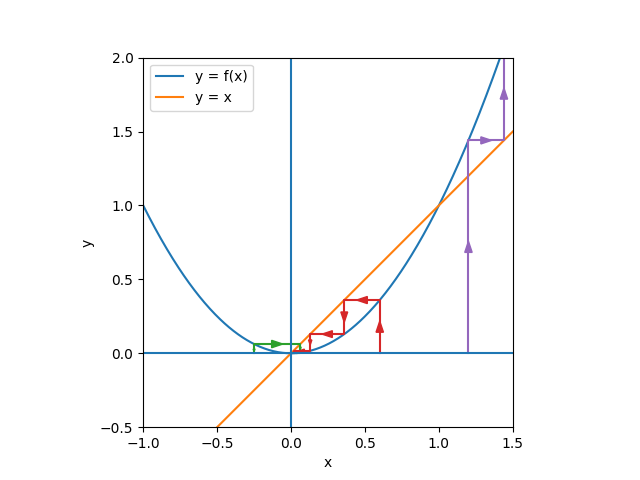
\includegraphics[width=\linewidth]{3.6 b gt -2.png}
			\caption{$-2 < b < 0$}
			\label{fig:3.6gt-2}
		\end{subfigure}
		\begin{subfigure}{.33\textwidth}
			\centering
			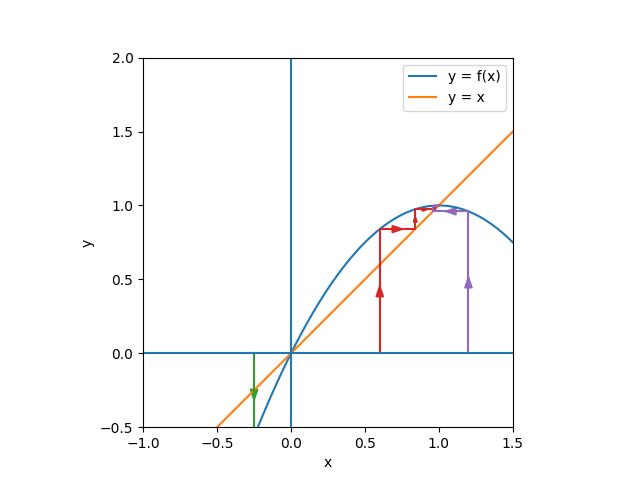
\includegraphics[width=\linewidth]{3.6 b gt 0.png}
			\caption{$0 < b < 2$}
			\label{fig:3.6gt0}
		\end{subfigure}
		\begin{subfigure}{.33\textwidth}
			\centering
			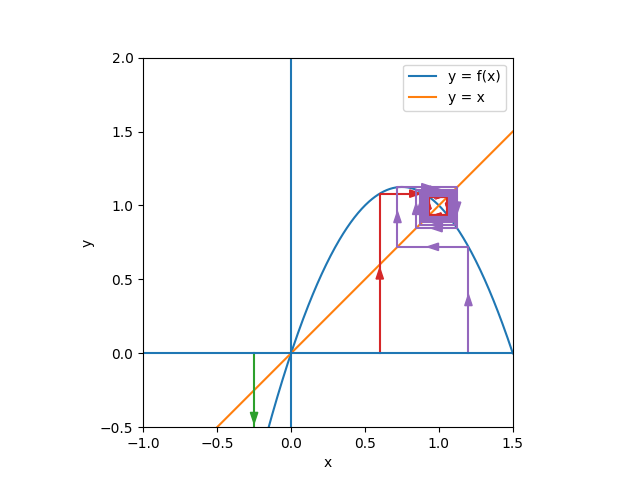
\includegraphics[width=\linewidth]{3.6 b eq 2.png}
			\caption{$b = 2$}
			\label{fig:3.6eq2}
		\end{subfigure}
		\begin{subfigure}{.33\textwidth}
			\centering
			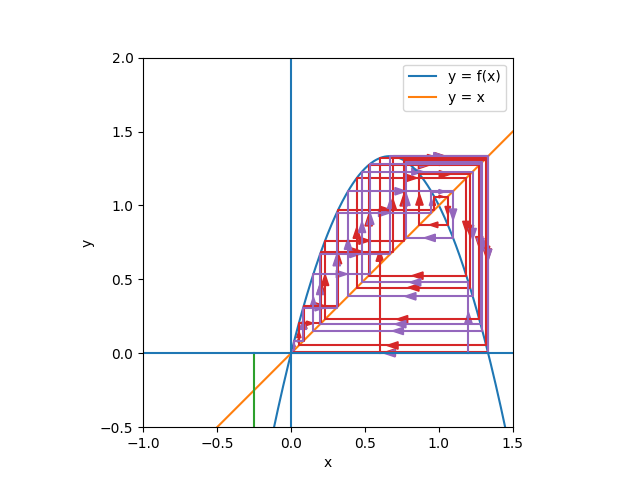
\includegraphics[width=\linewidth]{3.6 b gt 2.png}
			\caption{$b > 2$}
			\label{fig:3.6gt2}
		\end{subfigure}
		\caption{3.6 typical stair-step diagrams}
		\label{fig:3.6}
	\end{figure}
	
	\newpage
	
	\question*{Appendix}
	
	\lstinputlisting[language=Python, numbers=left, frame=single, basicstyle=\small\ttfamily, showstringspaces=false, caption={\lstinline{cbrt.py} -- cube root difference equation simulation}, label=lst:cbrt_sim]{cbrt.py}
	
	\lstinputlisting[language=Python, numbers=left, frame=single, basicstyle=\small\ttfamily, showstringspaces=false, caption={\lstinline{euler.py} -- Euler method for $\sqrt{2}$}, label=lst:euler]{euler.py}
	
	\newpage
	\lstinputlisting[language=Python, numbers=left, frame=single, basicstyle=\small\ttfamily, showstringspaces=false, caption={\lstinline{stairstep.py} -- Stair-step diagram generator}, label=lst:stairstep]{stairstep.py}
\end{document}